\hypertarget{_b___from_scattered_data_8c}{
\section{/home/mgh/LanlGeoMag/libLanlGeoMag/B\_\-FromScatteredData.c File Reference}
\label{_b___from_scattered_data_8c}\index{/home/mgh/LanlGeoMag/libLanlGeoMag/B\_\-FromScatteredData.c@{/home/mgh/LanlGeoMag/libLanlGeoMag/B\_\-FromScatteredData.c}}
}
{\tt \#include \char`\"{}Lgm/Lgm\_\-MagModelInfo.h\char`\"{}}\par
{\tt \#include \char`\"{}Lgm/Lgm\_\-Octree.h\char`\"{}}\par
{\tt \#include $<$stdlib.h$>$}\par
{\tt \#include $<$gsl/gsl\_\-matrix.h$>$}\par
{\tt \#include $<$gsl/gsl\_\-linalg.h$>$}\par


Include dependency graph for B\_\-FromScatteredData.c:\nopagebreak
\begin{figure}[H]
\begin{center}
\leavevmode
\includegraphics[width=420pt]{_b___from_scattered_data_8c__incl}
\end{center}
\end{figure}
\subsection*{Functions}
\begin{CompactItemize}
\item 
void \hyperlink{_b___from_scattered_data_8c_471b3b6d51257ae76e4a22fa1d2e6f67}{DFI\_\-BasisFuncLin} (double $\ast$b, \hyperlink{struct_lgm___vector}{Lgm\_\-Vector} $\ast$P)
\item 
void \hyperlink{_b___from_scattered_data_8c_373301cb1510ec76bf04e60f44cc26fa}{DFI\_\-FuncLin} (\hyperlink{struct_lgm___vector}{Lgm\_\-Vector} $\ast$P, gsl\_\-vector $\ast$C, \hyperlink{struct_lgm___vector}{Lgm\_\-Vector} $\ast$V)
\item 
void \hyperlink{_b___from_scattered_data_8c_63e1b24396d764119a3d822773af07cb}{DFI\_\-DivBasisFuncLin} (double $\ast$bdiv, \hyperlink{struct_lgm___vector}{Lgm\_\-Vector} $\ast$P)
\item 
void \hyperlink{_b___from_scattered_data_8c_9133efa4bdfaeed11bba2e75d25f29cf}{DFI\_\-BasisFunc} (double $\ast$b, \hyperlink{struct_lgm___vector}{Lgm\_\-Vector} $\ast$P)
\item 
void \hyperlink{_b___from_scattered_data_8c_3b380e0805c4cf987f1c07da8759ff86}{DFI\_\-Func} (\hyperlink{struct_lgm___vector}{Lgm\_\-Vector} $\ast$P, gsl\_\-vector $\ast$C, \hyperlink{struct_lgm___vector}{Lgm\_\-Vector} $\ast$V)
\item 
void \hyperlink{_b___from_scattered_data_8c_f267e6c987d5ca7607b0ad4af4d1b783}{DFI\_\-DivBasisFunc} (double $\ast$bdiv, \hyperlink{struct_lgm___vector}{Lgm\_\-Vector} $\ast$P)
\item 
int \hyperlink{_b___from_scattered_data_8c_d11ba2ce714d9d6e4b6dc532fabe87c9}{Lgm\_\-DivFreeInterp} (\hyperlink{struct_lgm___vector}{Lgm\_\-Vector} $\ast$q, \hyperlink{struct___lgm___octree_data}{Lgm\_\-OctreeData} $\ast$kNN, int K, \hyperlink{struct_lgm___vector}{Lgm\_\-Vector} $\ast$v)
\item 
int \hyperlink{_b___from_scattered_data_8c_b67853a5a2e18a5e252ffbe4ac3c9ea6}{Lgm\_\-DivFreeInterp2} (\hyperlink{struct_lgm___vector}{Lgm\_\-Vector} $\ast$q, \hyperlink{struct___lgm___octree_data}{Lgm\_\-OctreeData} $\ast$kNN, int K, \hyperlink{struct_lgm___vector}{Lgm\_\-Vector} $\ast$v)
\item 
int \hyperlink{_b___from_scattered_data_8c_5138e7f3fa8a67aa8ab528ba9cd606d2}{Lgm\_\-B\_\-FromScatteredData} (\hyperlink{struct_lgm___vector}{Lgm\_\-Vector} $\ast$v, \hyperlink{struct_lgm___vector}{Lgm\_\-Vector} $\ast$B, \hyperlink{struct_lgm___mag_model_info}{Lgm\_\-MagModelInfo} $\ast$Info)
\end{CompactItemize}


\subsection{Function Documentation}
\hypertarget{_b___from_scattered_data_8c_471b3b6d51257ae76e4a22fa1d2e6f67}{
\index{B\_\-FromScatteredData.c@{B\_\-FromScatteredData.c}!DFI\_\-BasisFuncLin@{DFI\_\-BasisFuncLin}}
\index{DFI\_\-BasisFuncLin@{DFI\_\-BasisFuncLin}!B_FromScatteredData.c@{B\_\-FromScatteredData.c}}
\subsubsection[{DFI\_\-BasisFuncLin}]{\setlength{\rightskip}{0pt plus 5cm}void DFI\_\-BasisFuncLin (double $\ast$ {\em b}, \/  {\bf Lgm\_\-Vector} $\ast$ {\em P})}}
\label{_b___from_scattered_data_8c_471b3b6d51257ae76e4a22fa1d2e6f67}




Definition at line 28 of file B\_\-FromScatteredData.c.

Here is the caller graph for this function:\nopagebreak
\begin{figure}[H]
\begin{center}
\leavevmode
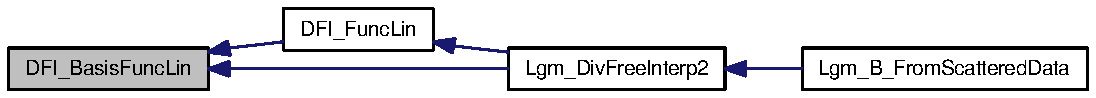
\includegraphics[width=281pt]{_b___from_scattered_data_8c_471b3b6d51257ae76e4a22fa1d2e6f67_icgraph}
\end{center}
\end{figure}
\hypertarget{_b___from_scattered_data_8c_373301cb1510ec76bf04e60f44cc26fa}{
\index{B\_\-FromScatteredData.c@{B\_\-FromScatteredData.c}!DFI\_\-FuncLin@{DFI\_\-FuncLin}}
\index{DFI\_\-FuncLin@{DFI\_\-FuncLin}!B_FromScatteredData.c@{B\_\-FromScatteredData.c}}
\subsubsection[{DFI\_\-FuncLin}]{\setlength{\rightskip}{0pt plus 5cm}void DFI\_\-FuncLin ({\bf Lgm\_\-Vector} $\ast$ {\em P}, \/  gsl\_\-vector $\ast$ {\em C}, \/  {\bf Lgm\_\-Vector} $\ast$ {\em V})}}
\label{_b___from_scattered_data_8c_373301cb1510ec76bf04e60f44cc26fa}




Definition at line 32 of file B\_\-FromScatteredData.c.

Here is the call graph for this function:\nopagebreak
\begin{figure}[H]
\begin{center}
\leavevmode
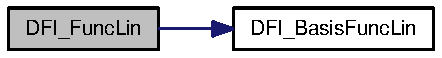
\includegraphics[width=124pt]{_b___from_scattered_data_8c_373301cb1510ec76bf04e60f44cc26fa_cgraph}
\end{center}
\end{figure}


Here is the caller graph for this function:\nopagebreak
\begin{figure}[H]
\begin{center}
\leavevmode
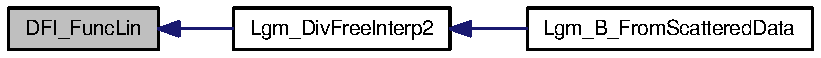
\includegraphics[width=215pt]{_b___from_scattered_data_8c_373301cb1510ec76bf04e60f44cc26fa_icgraph}
\end{center}
\end{figure}
\hypertarget{_b___from_scattered_data_8c_63e1b24396d764119a3d822773af07cb}{
\index{B\_\-FromScatteredData.c@{B\_\-FromScatteredData.c}!DFI\_\-DivBasisFuncLin@{DFI\_\-DivBasisFuncLin}}
\index{DFI\_\-DivBasisFuncLin@{DFI\_\-DivBasisFuncLin}!B_FromScatteredData.c@{B\_\-FromScatteredData.c}}
\subsubsection[{DFI\_\-DivBasisFuncLin}]{\setlength{\rightskip}{0pt plus 5cm}void DFI\_\-DivBasisFuncLin (double $\ast$ {\em bdiv}, \/  {\bf Lgm\_\-Vector} $\ast$ {\em P})}}
\label{_b___from_scattered_data_8c_63e1b24396d764119a3d822773af07cb}




Definition at line 42 of file B\_\-FromScatteredData.c.

Here is the caller graph for this function:\nopagebreak
\begin{figure}[H]
\begin{center}
\leavevmode
\includegraphics[width=235pt]{_b___from_scattered_data_8c_63e1b24396d764119a3d822773af07cb_icgraph}
\end{center}
\end{figure}
\hypertarget{_b___from_scattered_data_8c_9133efa4bdfaeed11bba2e75d25f29cf}{
\index{B\_\-FromScatteredData.c@{B\_\-FromScatteredData.c}!DFI\_\-BasisFunc@{DFI\_\-BasisFunc}}
\index{DFI\_\-BasisFunc@{DFI\_\-BasisFunc}!B_FromScatteredData.c@{B\_\-FromScatteredData.c}}
\subsubsection[{DFI\_\-BasisFunc}]{\setlength{\rightskip}{0pt plus 5cm}void DFI\_\-BasisFunc (double $\ast$ {\em b}, \/  {\bf Lgm\_\-Vector} $\ast$ {\em P})}}
\label{_b___from_scattered_data_8c_9133efa4bdfaeed11bba2e75d25f29cf}




Definition at line 58 of file B\_\-FromScatteredData.c.

Here is the caller graph for this function:\nopagebreak
\begin{figure}[H]
\begin{center}
\leavevmode
\includegraphics[width=267pt]{_b___from_scattered_data_8c_9133efa4bdfaeed11bba2e75d25f29cf_icgraph}
\end{center}
\end{figure}
\hypertarget{_b___from_scattered_data_8c_3b380e0805c4cf987f1c07da8759ff86}{
\index{B\_\-FromScatteredData.c@{B\_\-FromScatteredData.c}!DFI\_\-Func@{DFI\_\-Func}}
\index{DFI\_\-Func@{DFI\_\-Func}!B_FromScatteredData.c@{B\_\-FromScatteredData.c}}
\subsubsection[{DFI\_\-Func}]{\setlength{\rightskip}{0pt plus 5cm}void DFI\_\-Func ({\bf Lgm\_\-Vector} $\ast$ {\em P}, \/  gsl\_\-vector $\ast$ {\em C}, \/  {\bf Lgm\_\-Vector} $\ast$ {\em V})}}
\label{_b___from_scattered_data_8c_3b380e0805c4cf987f1c07da8759ff86}




Definition at line 65 of file B\_\-FromScatteredData.c.

Here is the call graph for this function:\nopagebreak
\begin{figure}[H]
\begin{center}
\leavevmode
\includegraphics[width=112pt]{_b___from_scattered_data_8c_3b380e0805c4cf987f1c07da8759ff86_cgraph}
\end{center}
\end{figure}


Here is the caller graph for this function:\nopagebreak
\begin{figure}[H]
\begin{center}
\leavevmode
\includegraphics[width=207pt]{_b___from_scattered_data_8c_3b380e0805c4cf987f1c07da8759ff86_icgraph}
\end{center}
\end{figure}
\hypertarget{_b___from_scattered_data_8c_f267e6c987d5ca7607b0ad4af4d1b783}{
\index{B\_\-FromScatteredData.c@{B\_\-FromScatteredData.c}!DFI\_\-DivBasisFunc@{DFI\_\-DivBasisFunc}}
\index{DFI\_\-DivBasisFunc@{DFI\_\-DivBasisFunc}!B_FromScatteredData.c@{B\_\-FromScatteredData.c}}
\subsubsection[{DFI\_\-DivBasisFunc}]{\setlength{\rightskip}{0pt plus 5cm}void DFI\_\-DivBasisFunc (double $\ast$ {\em bdiv}, \/  {\bf Lgm\_\-Vector} $\ast$ {\em P})}}
\label{_b___from_scattered_data_8c_f267e6c987d5ca7607b0ad4af4d1b783}




Definition at line 79 of file B\_\-FromScatteredData.c.\hypertarget{_b___from_scattered_data_8c_d11ba2ce714d9d6e4b6dc532fabe87c9}{
\index{B\_\-FromScatteredData.c@{B\_\-FromScatteredData.c}!Lgm\_\-DivFreeInterp@{Lgm\_\-DivFreeInterp}}
\index{Lgm\_\-DivFreeInterp@{Lgm\_\-DivFreeInterp}!B_FromScatteredData.c@{B\_\-FromScatteredData.c}}
\subsubsection[{Lgm\_\-DivFreeInterp}]{\setlength{\rightskip}{0pt plus 5cm}int Lgm\_\-DivFreeInterp ({\bf Lgm\_\-Vector} $\ast$ {\em q}, \/  {\bf Lgm\_\-OctreeData} $\ast$ {\em kNN}, \/  int {\em K}, \/  {\bf Lgm\_\-Vector} $\ast$ {\em v})}}
\label{_b___from_scattered_data_8c_d11ba2ce714d9d6e4b6dc532fabe87c9}




Definition at line 93 of file B\_\-FromScatteredData.c.

Here is the call graph for this function:\nopagebreak
\begin{figure}[H]
\begin{center}
\leavevmode
\includegraphics[width=180pt]{_b___from_scattered_data_8c_d11ba2ce714d9d6e4b6dc532fabe87c9_cgraph}
\end{center}
\end{figure}


Here is the caller graph for this function:\nopagebreak
\begin{figure}[H]
\begin{center}
\leavevmode
\includegraphics[width=159pt]{_b___from_scattered_data_8c_d11ba2ce714d9d6e4b6dc532fabe87c9_icgraph}
\end{center}
\end{figure}
\hypertarget{_b___from_scattered_data_8c_b67853a5a2e18a5e252ffbe4ac3c9ea6}{
\index{B\_\-FromScatteredData.c@{B\_\-FromScatteredData.c}!Lgm\_\-DivFreeInterp2@{Lgm\_\-DivFreeInterp2}}
\index{Lgm\_\-DivFreeInterp2@{Lgm\_\-DivFreeInterp2}!B_FromScatteredData.c@{B\_\-FromScatteredData.c}}
\subsubsection[{Lgm\_\-DivFreeInterp2}]{\setlength{\rightskip}{0pt plus 5cm}int Lgm\_\-DivFreeInterp2 ({\bf Lgm\_\-Vector} $\ast$ {\em q}, \/  {\bf Lgm\_\-OctreeData} $\ast$ {\em kNN}, \/  int {\em K}, \/  {\bf Lgm\_\-Vector} $\ast$ {\em v})}}
\label{_b___from_scattered_data_8c_b67853a5a2e18a5e252ffbe4ac3c9ea6}




Definition at line 294 of file B\_\-FromScatteredData.c.

Here is the call graph for this function:\nopagebreak
\begin{figure}[H]
\begin{center}
\leavevmode
\includegraphics[width=214pt]{_b___from_scattered_data_8c_b67853a5a2e18a5e252ffbe4ac3c9ea6_cgraph}
\end{center}
\end{figure}


Here is the caller graph for this function:\nopagebreak
\begin{figure}[H]
\begin{center}
\leavevmode
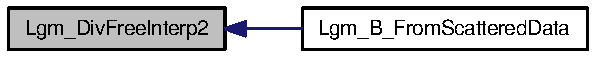
\includegraphics[width=161pt]{_b___from_scattered_data_8c_b67853a5a2e18a5e252ffbe4ac3c9ea6_icgraph}
\end{center}
\end{figure}
\hypertarget{_b___from_scattered_data_8c_5138e7f3fa8a67aa8ab528ba9cd606d2}{
\index{B\_\-FromScatteredData.c@{B\_\-FromScatteredData.c}!Lgm\_\-B\_\-FromScatteredData@{Lgm\_\-B\_\-FromScatteredData}}
\index{Lgm\_\-B\_\-FromScatteredData@{Lgm\_\-B\_\-FromScatteredData}!B_FromScatteredData.c@{B\_\-FromScatteredData.c}}
\subsubsection[{Lgm\_\-B\_\-FromScatteredData}]{\setlength{\rightskip}{0pt plus 5cm}int Lgm\_\-B\_\-FromScatteredData ({\bf Lgm\_\-Vector} $\ast$ {\em v}, \/  {\bf Lgm\_\-Vector} $\ast$ {\em B}, \/  {\bf Lgm\_\-MagModelInfo} $\ast$ {\em Info})}}
\label{_b___from_scattered_data_8c_5138e7f3fa8a67aa8ab528ba9cd606d2}




Definition at line 448 of file B\_\-FromScatteredData.c.

Here is the call graph for this function:\nopagebreak
\begin{figure}[H]
\begin{center}
\leavevmode
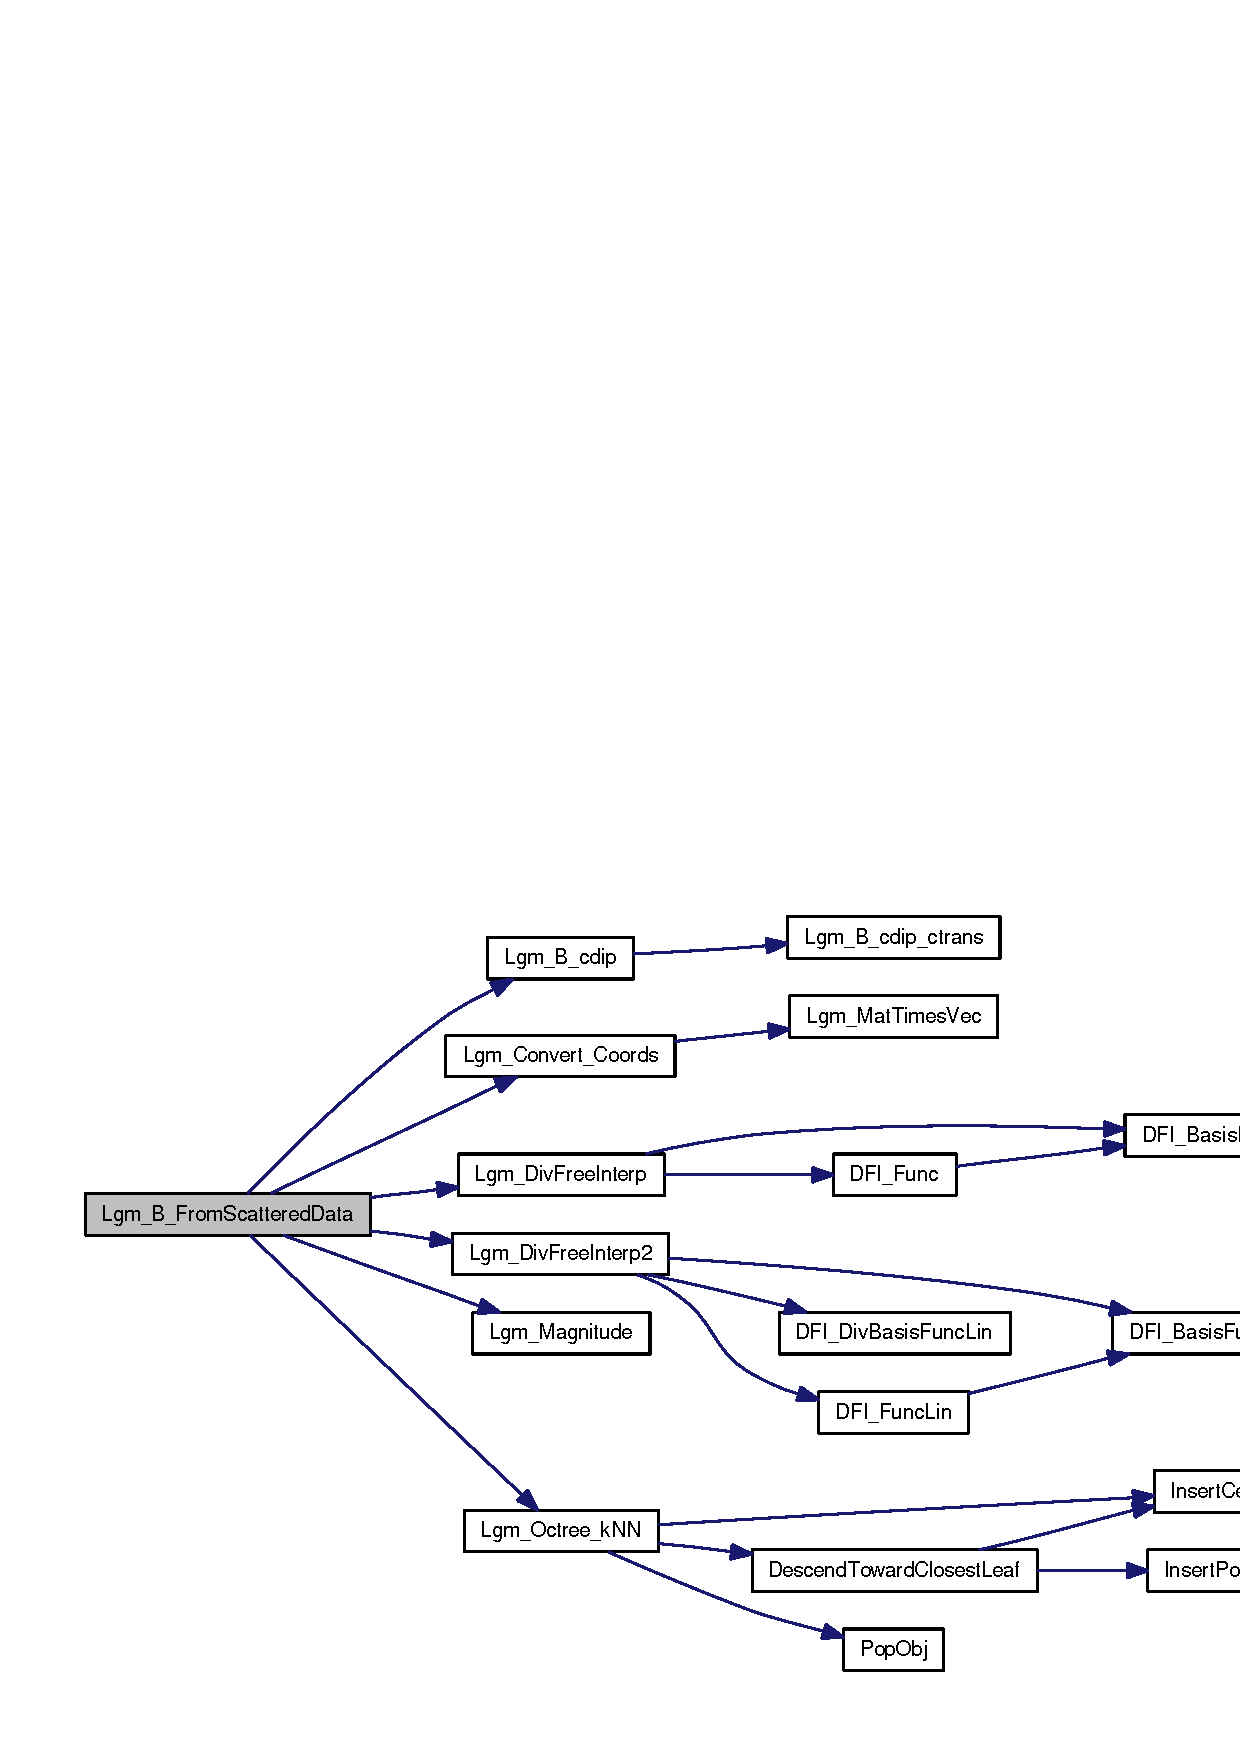
\includegraphics[width=360pt]{_b___from_scattered_data_8c_5138e7f3fa8a67aa8ab528ba9cd606d2_cgraph}
\end{center}
\end{figure}
